\documentclass{standalone}
\usepackage{tikz}
\usetikzlibrary{patterns, positioning}
\usepackage[sfdefault]{ClearSans} %% option 'sfdefault' activates Clear Sans as the default text font
\usepackage[T1]{fontenc}

\begin{document}
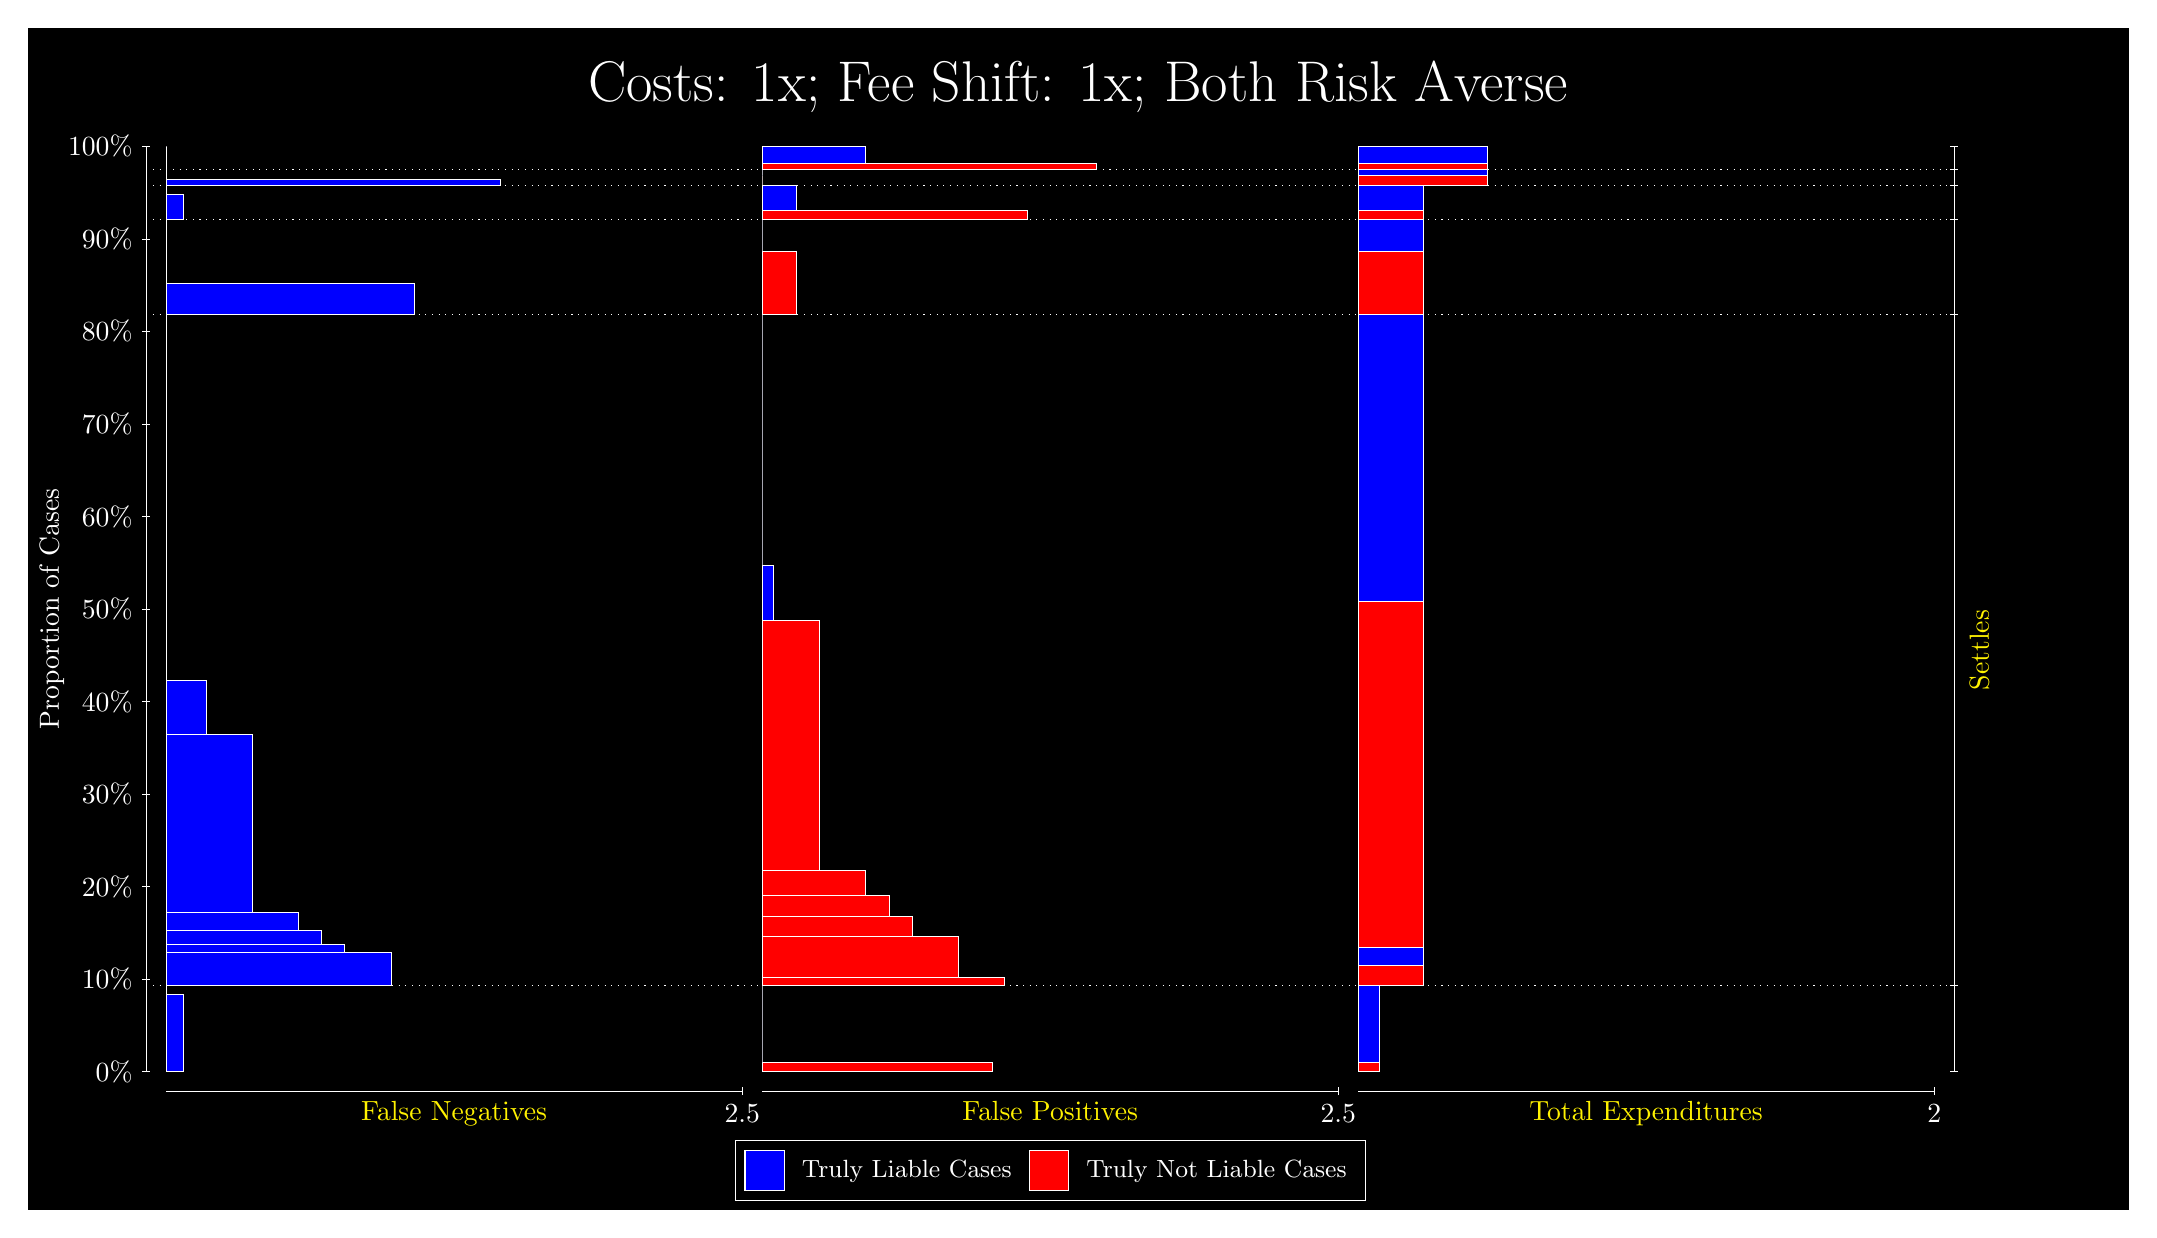
\begin{tikzpicture}
\draw[fill=black] (0,0) rectangle (26.667,15);
\draw[text=white] (0,13.5) rectangle (26.667,15) node[midway] {\huge Costs: 1x; Fee Shift: 1x; Both Risk Averse};
\draw[white, very thin] (1.5,1.75) -- (1.5,13.5);
\node[rotate=90, text=white, anchor=center] at (0.3, 7.625) {Proportion of Cases};
\draw[white, very thin] (1.45,1.75) -- (1.55,1.75);
\node[text=white, anchor=east] at (1.45, 1.75) {0\%};
\draw[white, very thin] (1.45,2.925) -- (1.55,2.925);
\node[text=white, anchor=east] at (1.45, 2.925) {10\%};
\draw[white, very thin] (1.45,4.1) -- (1.55,4.1);
\node[text=white, anchor=east] at (1.45, 4.1) {20\%};
\draw[white, very thin] (1.45,5.275) -- (1.55,5.275);
\node[text=white, anchor=east] at (1.45, 5.275) {30\%};
\draw[white, very thin] (1.45,6.45) -- (1.55,6.45);
\node[text=white, anchor=east] at (1.45, 6.45) {40\%};
\draw[white, very thin] (1.45,7.625) -- (1.55,7.625);
\node[text=white, anchor=east] at (1.45, 7.625) {50\%};
\draw[white, very thin] (1.45,8.8) -- (1.55,8.8);
\node[text=white, anchor=east] at (1.45, 8.8) {60\%};
\draw[white, very thin] (1.45,9.975) -- (1.55,9.975);
\node[text=white, anchor=east] at (1.45, 9.975) {70\%};
\draw[white, very thin] (1.45,11.15) -- (1.55,11.15);
\node[text=white, anchor=east] at (1.45, 11.15) {80\%};
\draw[white, very thin] (1.45,12.325) -- (1.55,12.325);
\node[text=white, anchor=east] at (1.45, 12.325) {90\%};
\draw[white, very thin] (1.45,13.5) -- (1.55,13.5);
\node[text=white, anchor=east] at (1.45, 13.5) {100\%};

\draw[white, very thin] (24.457,1.75) -- (24.457,13.5);
\draw[white, very thin] (24.407,1.75) -- (24.507,1.75);
\node[anchor=west] at (24.407, 1.75) {};
\draw[white, very thin] (24.407,2.8431) -- (24.507,2.8431);
\node[anchor=west] at (24.407, 2.8431) {};
\draw[white, very thin] (24.407,11.365) -- (24.507,11.365);
\node[anchor=west] at (24.407, 11.365) {};
\draw[white, very thin] (24.407,12.568) -- (24.507,12.568);
\node[anchor=west] at (24.407, 12.568) {};
\draw[white, very thin] (24.407,13.006) -- (24.507,13.006);
\node[anchor=west] at (24.407, 13.006) {};
\draw[white, very thin] (24.407,13.209) -- (24.507,13.209);
\node[anchor=west] at (24.407, 13.209) {};
\draw[white, very thin] (24.407,13.5) -- (24.507,13.5);
\node[anchor=west] at (24.407, 13.5) {};

\draw[white, very thin, fill=blue] (1.75,1.75) rectangle (1.9696,2.7281);
\draw[white, very thin, fill=red] (1.75,2.7281) rectangle (1.75,2.8431);
\draw[white, very thin, fill=blue] (1.75,2.8431) rectangle (4.6044,3.2588);
\draw[white, very thin, fill=blue] (1.75,3.2588) rectangle (4.0188,3.3724);
\draw[white, very thin, fill=blue] (1.75,3.3724) rectangle (3.7261,3.5387);
\draw[white, very thin, fill=blue] (1.75,3.5387) rectangle (3.4333,3.7745);
\draw[white, very thin, fill=blue] (1.75,3.7745) rectangle (2.8478,6.0287);
\draw[white, very thin, fill=blue] (1.75,6.0287) rectangle (2.2623,6.7242);
\draw[white, very thin, fill=red] (1.75,6.7242) rectangle (1.75,11.365);
\draw[white, very thin, fill=blue] (1.75,11.365) rectangle (4.8971,11.766);
\draw[white, very thin, fill=red] (1.75,11.766) rectangle (1.75,12.568);
\draw[white, very thin, fill=blue] (1.75,12.568) rectangle (1.9696,12.892);
\draw[white, very thin, fill=red] (1.75,12.892) rectangle (1.75,13.006);
\draw[white, very thin, fill=blue] (1.75,13.006) rectangle (5.9949,13.086);
\draw[white, very thin, fill=red] (1.75,13.086) rectangle (1.75,13.209);
\draw[white, very thin, fill=red] (1.75,13.209) rectangle (1.75,13.29);
\draw[white, very thin, fill=blue] (1.75,13.29) rectangle (1.75,13.5);
\draw[white, very thin, fill=red] (9.3189,1.75) rectangle (12.246,1.865);
\draw[white, very thin, fill=blue] (9.3189,1.865) rectangle (9.3189,2.8431);
\draw[white, very thin, fill=red] (9.3189,2.8431) rectangle (12.393,2.9531);
\draw[white, very thin, fill=red] (9.3189,2.9531) rectangle (11.807,3.4657);
\draw[white, very thin, fill=red] (9.3189,3.4657) rectangle (11.222,3.7177);
\draw[white, very thin, fill=red] (9.3189,3.7177) rectangle (10.929,3.988);
\draw[white, very thin, fill=red] (9.3189,3.988) rectangle (10.636,4.3119);
\draw[white, very thin, fill=red] (9.3189,4.3119) rectangle (10.051,7.4835);
\draw[white, very thin, fill=blue] (9.3189,7.4835) rectangle (9.4652,8.179);
\draw[white, very thin, fill=blue] (9.3189,8.179) rectangle (9.3189,11.365);
\draw[white, very thin, fill=red] (9.3189,11.365) rectangle (9.758,12.167);
\draw[white, very thin, fill=blue] (9.3189,12.167) rectangle (9.3189,12.568);
\draw[white, very thin, fill=red] (9.3189,12.568) rectangle (12.686,12.682);
\draw[white, very thin, fill=blue] (9.3189,12.682) rectangle (9.758,13.006);
\draw[white, very thin, fill=red] (9.3189,13.006) rectangle (9.3189,13.129);
\draw[white, very thin, fill=blue] (9.3189,13.129) rectangle (9.3189,13.209);
\draw[white, very thin, fill=red] (9.3189,13.209) rectangle (13.564,13.29);
\draw[white, very thin, fill=blue] (9.3189,13.29) rectangle (10.636,13.5);
\draw[white, very thin, fill=red] (16.888,1.75) rectangle (17.162,1.865);
\draw[white, very thin, fill=blue] (16.888,1.865) rectangle (17.162,2.8431);
\draw[white, very thin, fill=red] (16.888,2.8431) rectangle (17.711,3.0951);
\draw[white, very thin, fill=blue] (16.888,3.0951) rectangle (17.711,3.3309);
\draw[white, very thin, fill=red] (16.888,3.3309) rectangle (17.711,7.7193);
\draw[white, very thin, fill=blue] (16.888,7.7193) rectangle (17.711,11.365);
\draw[white, very thin, fill=red] (16.888,11.365) rectangle (17.711,12.167);
\draw[white, very thin, fill=blue] (16.888,12.167) rectangle (17.711,12.568);
\draw[white, very thin, fill=red] (16.888,12.568) rectangle (17.711,12.682);
\draw[white, very thin, fill=blue] (16.888,12.682) rectangle (17.711,13.006);
\draw[white, very thin, fill=red] (16.888,13.006) rectangle (18.534,13.129);
\draw[white, very thin, fill=blue] (16.888,13.129) rectangle (18.534,13.209);
\draw[white, very thin, fill=red] (16.888,13.209) rectangle (18.534,13.29);
\draw[white, very thin, fill=blue] (16.888,13.29) rectangle (18.534,13.5);
\draw[white, dotted] (1.5,2.8431) -- (24.457,2.8431);
\draw[white, dotted] (1.5,11.365) -- (24.457,11.365);
\draw[white, dotted] (1.5,12.568) -- (24.457,12.568);
\draw[white, dotted] (1.5,13.006) -- (24.457,13.006);
\draw[white, dotted] (1.5,13.209) -- (24.457,13.209);
\draw[white, very thin] (1.75,1.5) -- (9.0689,1.5);
\node[text=yellow, anchor=north] at (5.4094, 1.5) {False Negatives};
\draw[white, very thin] (9.0689,1.45) -- (9.0689,1.55);
\node[text=white, anchor=north] at (9.0689, 1.45) {2.5};

\draw[white, very thin] (9.3189,1.5) -- (16.638,1.5);
\node[text=yellow, anchor=north] at (12.978, 1.5) {False Positives};
\draw[white, very thin] (16.638,1.45) -- (16.638,1.55);
\node[text=white, anchor=north] at (16.638, 1.45) {2.5};

\draw[white, very thin] (16.888,1.5) -- (24.207,1.5);
\node[text=yellow, anchor=north] at (20.547, 1.5) {Total Expenditures};
\draw[white, very thin] (24.207,1.45) -- (24.207,1.55);
\node[text=white, anchor=north] at (24.207, 1.45) {2};


\node[text=yellow, centered, rotate=90] at (24.777, 7.1038) {Settles};





\draw (12.978300999999998,1.5) node[draw=none] (baseCoordinate) {};
\begin{scope}[align=center]
        \matrix[scale=0.5, draw=white, below=0.5cm of baseCoordinate, nodes={draw}, column sep=0.1cm]{
            \node[rectangle, draw, minimum width=0.5cm, minimum height=0.5cm, fill=blue] {}; &
            \node[draw=none, font=\small, text=white] (B) {Truly Liable Cases}; &
            \node[rectangle, draw, minimum width=0.5cm, minimum height=0.5cm, fill=red] {}; &
            \node[draw=none, font=\small, text=white] (B) {Truly Not Liable Cases}; \\
            };
\end{scope}

\end{tikzpicture}
\end{document}